\chapter{Theme Token Vocabulary}\label{record-028}

\noindent{\footnotesize\color{BookMuted}\path{docs/design-system/theme-tokens.md}\par}\smallskip

This document locks down the canonical token vocabulary for Bijou.

The \texttt{T\allowbreak{}h\allowbreak{}e\allowbreak{}m\allowbreak{}e} type in \href{https://github.com/flyingrobots/bijou/blob/cbd70612140e7a450d764b3c7be1c6af878b99bc/packages/bijou/src/core/theme/tokens.ts}{\texttt{p\allowbreak{}a\allowbreak{}c\allowbreak{}k\allowbreak{}a\allowbreak{}g\allowbreak{}e\allowbreak{}s\allowbreak{}/\allowbreak{}b\allowbreak{}i\allowbreak{}j\allowbreak{}o\allowbreak{}u\allowbreak{}/\allowbreak{}s\allowbreak{}r\allowbreak{}c\allowbreak{}/\allowbreak{}c\allowbreak{}o\allowbreak{}r\allowbreak{}e\allowbreak{}/\allowbreak{}t\allowbreak{}h\allowbreak{}e\allowbreak{}m\allowbreak{}e\allowbreak{}/\allowbreak{}t\allowbreak{}o\allowbreak{}k\allowbreak{}e\allowbreak{}n\allowbreak{}s\allowbreak{}.\allowbreak{}t\allowbreak{}s}} is the API truth. This page is the doctrine truth: it defines what each token family is for, what first-party components should prefer, and what counts as misuse.

\section{Why this exists}\label{record-028-why-this-exists}

Bijou already ships a typed token model:

\begin{itemize}
\tightlist
\item
  \texttt{s\allowbreak{}e\allowbreak{}m\allowbreak{}a\allowbreak{}n\allowbreak{}t\allowbreak{}i\allowbreak{}c}
\item
  \texttt{s\allowbreak{}u\allowbreak{}r\allowbreak{}f\allowbreak{}a\allowbreak{}c\allowbreak{}e}
\item
  \texttt{b\allowbreak{}o\allowbreak{}r\allowbreak{}d\allowbreak{}e\allowbreak{}r}
\item
  \texttt{u\allowbreak{}i}
\item
  \texttt{s\allowbreak{}t\allowbreak{}a\allowbreak{}t\allowbreak{}u\allowbreak{}s}
\item
  \texttt{g\allowbreak{}r\allowbreak{}a\allowbreak{}d\allowbreak{}i\allowbreak{}e\allowbreak{}n\allowbreak{}t}
\end{itemize}

What was missing was the rulebook. Without one, component authors end up choosing tokens by ``what looks right in this preset'' instead of by semantic job, and the design system drifts into an untyped color bucket.

\section{Core rule}\label{record-028-core-rule}

Choose tokens by meaning, not by color.

If a component needs a green foreground because it means ``success'', use a success token. Do not reach for whichever family currently contains a green hex value in the active preset.

\section{Canonical families}\label{record-028-canonical-families}

\subsection{\texorpdfstring{\texttt{s\allowbreak{}e\allowbreak{}m\allowbreak{}a\allowbreak{}n\allowbreak{}t\allowbreak{}i\allowbreak{}c}}{}}\label{record-028-semantic}

Use \texttt{s\allowbreak{}e\allowbreak{}m\allowbreak{}a\allowbreak{}n\allowbreak{}t\allowbreak{}i\allowbreak{}c} for general foreground meaning and emphasis inside a component.

This is the default family for:

\begin{itemize}
\tightlist
\item
  primary text emphasis
\item
  supporting or muted text
\item
  active or focused emphasis inside a component
\item
  generic semantic cues that are not domain statuses
\end{itemize}

Built-in keys:

\begin{itemize}
\tightlist
\item
  \texttt{p\allowbreak{}r\allowbreak{}i\allowbreak{}m\allowbreak{}a\allowbreak{}r\allowbreak{}y}
\item
  \texttt{m\allowbreak{}u\allowbreak{}t\allowbreak{}e\allowbreak{}d}
\item
  \texttt{a\allowbreak{}c\allowbreak{}c\allowbreak{}e\allowbreak{}n\allowbreak{}t}
\item
  \texttt{s\allowbreak{}u\allowbreak{}c\allowbreak{}c\allowbreak{}e\allowbreak{}s\allowbreak{}s}
\item
  \texttt{e\allowbreak{}r\allowbreak{}r\allowbreak{}o\allowbreak{}r}
\item
  \texttt{w\allowbreak{}a\allowbreak{}r\allowbreak{}n\allowbreak{}i\allowbreak{}n\allowbreak{}g}
\item
  \texttt{i\allowbreak{}n\allowbreak{}f\allowbreak{}o}
\end{itemize}

House rules:

\begin{itemize}
\tightlist
\item
  prefer \texttt{s\allowbreak{}e\allowbreak{}m\allowbreak{}a\allowbreak{}n\allowbreak{}t\allowbreak{}i\allowbreak{}c\allowbreak{}.\allowbreak{}p\allowbreak{}r\allowbreak{}i\allowbreak{}m\allowbreak{}a\allowbreak{}r\allowbreak{}y} for deliberate foreground emphasis
\item
  prefer \texttt{s\allowbreak{}e\allowbreak{}m\allowbreak{}a\allowbreak{}n\allowbreak{}t\allowbreak{}i\allowbreak{}c\allowbreak{}.\allowbreak{}m\allowbreak{}u\allowbreak{}t\allowbreak{}e\allowbreak{}d} for metadata, hints, and supporting text
\item
  prefer \texttt{s\allowbreak{}e\allowbreak{}m\allowbreak{}a\allowbreak{}n\allowbreak{}t\allowbreak{}i\allowbreak{}c\allowbreak{}.\allowbreak{}a\allowbreak{}c\allowbreak{}c\allowbreak{}e\allowbreak{}n\allowbreak{}t} for local active/focused affordances inside a component
\item
  do not use \texttt{s\allowbreak{}e\allowbreak{}m\allowbreak{}a\allowbreak{}n\allowbreak{}t\allowbreak{}i\allowbreak{}c\allowbreak{}.\allowbreak{}*} as a generic background-fill family
\end{itemize}

\subsection{\texorpdfstring{\texttt{s\allowbreak{}u\allowbreak{}r\allowbreak{}f\allowbreak{}a\allowbreak{}c\allowbreak{}e}}{}}\label{record-028-surface}

Use \texttt{s\allowbreak{}u\allowbreak{}r\allowbreak{}f\allowbreak{}a\allowbreak{}c\allowbreak{}e} for containment, fill, elevation, and interruption level.

This is the default family for:

\begin{itemize}
\tightlist
\item
  panel and card backgrounds
\item
  sidebars and secondary rails
\item
  elevated regions
\item
  overlays, drawers, and modal fills
\item
  muted or disabled regions
\end{itemize}

Built-in keys:

\begin{itemize}
\tightlist
\item
  \texttt{p\allowbreak{}r\allowbreak{}i\allowbreak{}m\allowbreak{}a\allowbreak{}r\allowbreak{}y}
\item
  \texttt{s\allowbreak{}e\allowbreak{}c\allowbreak{}o\allowbreak{}n\allowbreak{}d\allowbreak{}a\allowbreak{}r\allowbreak{}y}
\item
  \texttt{e\allowbreak{}l\allowbreak{}e\allowbreak{}v\allowbreak{}a\allowbreak{}t\allowbreak{}e\allowbreak{}d}
\item
  \texttt{o\allowbreak{}v\allowbreak{}e\allowbreak{}r\allowbreak{}l\allowbreak{}a\allowbreak{}y}
\item
  \texttt{m\allowbreak{}u\allowbreak{}t\allowbreak{}e\allowbreak{}d}
\end{itemize}

House rules:

\begin{itemize}
\tightlist
\item
  treat \texttt{s\allowbreak{}u\allowbreak{}r\allowbreak{}f\allowbreak{}a\allowbreak{}c\allowbreak{}e\allowbreak{}.\allowbreak{}p\allowbreak{}r\allowbreak{}i\allowbreak{}m\allowbreak{}a\allowbreak{}r\allowbreak{}y} as the default content-region fill
\item
  treat \texttt{s\allowbreak{}u\allowbreak{}r\allowbreak{}f\allowbreak{}a\allowbreak{}c\allowbreak{}e\allowbreak{}.\allowbreak{}s\allowbreak{}e\allowbreak{}c\allowbreak{}o\allowbreak{}n\allowbreak{}d\allowbreak{}a\allowbreak{}r\allowbreak{}y} as the secondary-pane or sidebar fill
\item
  treat \texttt{s\allowbreak{}u\allowbreak{}r\allowbreak{}f\allowbreak{}a\allowbreak{}c\allowbreak{}e\allowbreak{}.\allowbreak{}e\allowbreak{}l\allowbreak{}e\allowbreak{}v\allowbreak{}a\allowbreak{}t\allowbreak{}e\allowbreak{}d} as the default fill for bounded contained objects
\item
  treat \texttt{s\allowbreak{}u\allowbreak{}r\allowbreak{}f\allowbreak{}a\allowbreak{}c\allowbreak{}e\allowbreak{}.\allowbreak{}o\allowbreak{}v\allowbreak{}e\allowbreak{}r\allowbreak{}l\allowbreak{}a\allowbreak{}y} as the interruption or overlay fill
\item
  treat \texttt{s\allowbreak{}u\allowbreak{}r\allowbreak{}f\allowbreak{}a\allowbreak{}c\allowbreak{}e\allowbreak{}.\allowbreak{}m\allowbreak{}u\allowbreak{}t\allowbreak{}e\allowbreak{}d} as the disabled, inset, or de-emphasized fill
\item
  do not use surface choice to smuggle status meaning
\end{itemize}

\subsection{\texorpdfstring{\texttt{b\allowbreak{}o\allowbreak{}r\allowbreak{}d\allowbreak{}e\allowbreak{}r}}{}}\label{record-028-border}

Use \texttt{b\allowbreak{}o\allowbreak{}r\allowbreak{}d\allowbreak{}e\allowbreak{}r} for structure, grouping, and boundary emphasis.

This is the default family for:

\begin{itemize}
\tightlist
\item
  box outlines
\item
  separators that need tokenized color
\item
  severity-bearing frames when the frame itself carries meaning
\end{itemize}

Built-in keys:

\begin{itemize}
\tightlist
\item
  \texttt{p\allowbreak{}r\allowbreak{}i\allowbreak{}m\allowbreak{}a\allowbreak{}r\allowbreak{}y}
\item
  \texttt{s\allowbreak{}e\allowbreak{}c\allowbreak{}o\allowbreak{}n\allowbreak{}d\allowbreak{}a\allowbreak{}r\allowbreak{}y}
\item
  \texttt{s\allowbreak{}u\allowbreak{}c\allowbreak{}c\allowbreak{}e\allowbreak{}s\allowbreak{}s}
\item
  \texttt{w\allowbreak{}a\allowbreak{}r\allowbreak{}n\allowbreak{}i\allowbreak{}n\allowbreak{}g}
\item
  \texttt{e\allowbreak{}r\allowbreak{}r\allowbreak{}o\allowbreak{}r}
\item
  \texttt{m\allowbreak{}u\allowbreak{}t\allowbreak{}e\allowbreak{}d}
\end{itemize}

House rules:

\begin{itemize}
\tightlist
\item
  prefer \texttt{b\allowbreak{}o\allowbreak{}r\allowbreak{}d\allowbreak{}e\allowbreak{}r\allowbreak{}.\allowbreak{}m\allowbreak{}u\allowbreak{}t\allowbreak{}e\allowbreak{}d} for ordinary structure
\item
  use \texttt{b\allowbreak{}o\allowbreak{}r\allowbreak{}d\allowbreak{}e\allowbreak{}r\allowbreak{}.\allowbreak{}p\allowbreak{}r\allowbreak{}i\allowbreak{}m\allowbreak{}a\allowbreak{}r\allowbreak{}y} or \texttt{b\allowbreak{}o\allowbreak{}r\allowbreak{}d\allowbreak{}e\allowbreak{}r\allowbreak{}.\allowbreak{}s\allowbreak{}e\allowbreak{}c\allowbreak{}o\allowbreak{}n\allowbreak{}d\allowbreak{}a\allowbreak{}r\allowbreak{}y} for stronger non-status grouping
\item
  use status-colored borders only when the border itself is part of the state
\item
  do not use warning/error borders as decoration
\end{itemize}

\subsection{\texorpdfstring{\texttt{u\allowbreak{}i}}{}}\label{record-028-ui}

Use \texttt{u\allowbreak{}i} for runtime chrome and reusable system affordances that do not belong to domain data.

This is the default family for:

\begin{itemize}
\tightlist
\item
  cursor or selection chrome owned by the shell/runtime
\item
  focused pane gutters owned by reusable shell frames
\item
  scrollbars and tracks
\item
  section headers
\item
  logos or branded shell marks
\item
  table headers when they are part of reusable framework chrome
\item
  empty tracks and similar UI scaffolding
\end{itemize}

Built-in keys:

\begin{itemize}
\tightlist
\item
  \texttt{c\allowbreak{}u\allowbreak{}r\allowbreak{}s\allowbreak{}o\allowbreak{}r}
\item
  \texttt{f\allowbreak{}o\allowbreak{}c\allowbreak{}u\allowbreak{}s\allowbreak{}G\allowbreak{}u\allowbreak{}t\allowbreak{}t\allowbreak{}e\allowbreak{}r}
\item
  \texttt{s\allowbreak{}c\allowbreak{}r\allowbreak{}o\allowbreak{}l\allowbreak{}l\allowbreak{}T\allowbreak{}h\allowbreak{}u\allowbreak{}m\allowbreak{}b}
\item
  \texttt{s\allowbreak{}c\allowbreak{}r\allowbreak{}o\allowbreak{}l\allowbreak{}l\allowbreak{}T\allowbreak{}r\allowbreak{}a\allowbreak{}c\allowbreak{}k}
\item
  \texttt{s\allowbreak{}e\allowbreak{}c\allowbreak{}t\allowbreak{}i\allowbreak{}o\allowbreak{}n\allowbreak{}H\allowbreak{}e\allowbreak{}a\allowbreak{}d\allowbreak{}e\allowbreak{}r}
\item
  \texttt{l\allowbreak{}o\allowbreak{}g\allowbreak{}o}
\item
  \texttt{t\allowbreak{}a\allowbreak{}b\allowbreak{}l\allowbreak{}e\allowbreak{}H\allowbreak{}e\allowbreak{}a\allowbreak{}d\allowbreak{}e\allowbreak{}r}
\item
  \texttt{t\allowbreak{}r\allowbreak{}a\allowbreak{}c\allowbreak{}k\allowbreak{}E\allowbreak{}m\allowbreak{}p\allowbreak{}t\allowbreak{}y}
\end{itemize}

House rules:

\begin{itemize}
\tightlist
\item
  reserve \texttt{u\allowbreak{}i\allowbreak{}.\allowbreak{}*} for framework/runtime chrome, not business-domain statuses
\item
  prefer a dedicated \texttt{u\allowbreak{}i} token when the same affordance recurs across shells
\item
  use \texttt{u\allowbreak{}i\allowbreak{}.\allowbreak{}f\allowbreak{}o\allowbreak{}c\allowbreak{}u\allowbreak{}s\allowbreak{}G\allowbreak{}u\allowbreak{}t\allowbreak{}t\allowbreak{}e\allowbreak{}r} for focused shell pane gutters; use \texttt{s\allowbreak{}e\allowbreak{}m\allowbreak{}a\allowbreak{}n\allowbreak{}t\allowbreak{}i\allowbreak{}c\allowbreak{}.\allowbreak{}a\allowbreak{}c\allowbreak{}c\allowbreak{}e\allowbreak{}n\allowbreak{}t} for local active emphasis inside a component
\item
  do not use \texttt{u\allowbreak{}i\allowbreak{}.\allowbreak{}*} as a back door for arbitrary one-off component colors
\end{itemize}

\subsection{\texorpdfstring{\texttt{s\allowbreak{}t\allowbreak{}a\allowbreak{}t\allowbreak{}u\allowbreak{}s}}{}}\label{record-028-status}

Use \texttt{s\allowbreak{}t\allowbreak{}a\allowbreak{}t\allowbreak{}u\allowbreak{}s} for explicit state labels and indicators attached to an object, process, or record.

This is the default family for:

\begin{itemize}
\tightlist
\item
  badges
\item
  timeline states
\item
  health/readiness indicators
\item
  process states such as pending or active
\end{itemize}

Built-in keys:

\begin{itemize}
\tightlist
\item
  \texttt{s\allowbreak{}u\allowbreak{}c\allowbreak{}c\allowbreak{}e\allowbreak{}s\allowbreak{}s}
\item
  \texttt{e\allowbreak{}r\allowbreak{}r\allowbreak{}o\allowbreak{}r}
\item
  \texttt{w\allowbreak{}a\allowbreak{}r\allowbreak{}n\allowbreak{}i\allowbreak{}n\allowbreak{}g}
\item
  \texttt{i\allowbreak{}n\allowbreak{}f\allowbreak{}o}
\item
  \texttt{p\allowbreak{}e\allowbreak{}n\allowbreak{}d\allowbreak{}i\allowbreak{}n\allowbreak{}g}
\item
  \texttt{a\allowbreak{}c\allowbreak{}t\allowbreak{}i\allowbreak{}v\allowbreak{}e}
\item
  \texttt{m\allowbreak{}u\allowbreak{}t\allowbreak{}e\allowbreak{}d}
\end{itemize}

House rules:

\begin{itemize}
\tightlist
\item
  use \texttt{s\allowbreak{}t\allowbreak{}a\allowbreak{}t\allowbreak{}u\allowbreak{}s\allowbreak{}.\allowbreak{}*} when the UI is naming or signaling a real status
\item
  prefer \texttt{s\allowbreak{}t\allowbreak{}a\allowbreak{}t\allowbreak{}u\allowbreak{}s\allowbreak{}.\allowbreak{}p\allowbreak{}e\allowbreak{}n\allowbreak{}d\allowbreak{}i\allowbreak{}n\allowbreak{}g} and \texttt{s\allowbreak{}t\allowbreak{}a\allowbreak{}t\allowbreak{}u\allowbreak{}s\allowbreak{}.\allowbreak{}a\allowbreak{}c\allowbreak{}t\allowbreak{}i\allowbreak{}v\allowbreak{}e} over reusing accent/focus tokens
\item
  do not use \texttt{s\allowbreak{}t\allowbreak{}a\allowbreak{}t\allowbreak{}u\allowbreak{}s\allowbreak{}.\allowbreak{}*} for focus, hover, or generic ``selected'' styling
\end{itemize}

\subsection{\texorpdfstring{\texttt{g\allowbreak{}r\allowbreak{}a\allowbreak{}d\allowbreak{}i\allowbreak{}e\allowbreak{}n\allowbreak{}t}}{}}\label{record-028-gradient}

Use \texttt{g\allowbreak{}r\allowbreak{}a\allowbreak{}d\allowbreak{}i\allowbreak{}e\allowbreak{}n\allowbreak{}t} for rare multi-stop emphasis that is intentionally decorative or specialized.

Built-in keys:

\begin{itemize}
\tightlist
\item
  \texttt{b\allowbreak{}r\allowbreak{}a\allowbreak{}n\allowbreak{}d}
\item
  \texttt{p\allowbreak{}r\allowbreak{}o\allowbreak{}g\allowbreak{}r\allowbreak{}e\allowbreak{}s\allowbreak{}s}
\end{itemize}

House rules:

\begin{itemize}
\tightlist
\item
  gradients are optional emphasis, not required meaning
\item
  never make critical status, navigation, or instructions depend on a gradient
\item
  prefer \texttt{g\allowbreak{}r\allowbreak{}a\allowbreak{}d\allowbreak{}i\allowbreak{}e\allowbreak{}n\allowbreak{}t\allowbreak{}.\allowbreak{}p\allowbreak{}r\allowbreak{}o\allowbreak{}g\allowbreak{}r\allowbreak{}e\allowbreak{}s\allowbreak{}s} only when the component is actually showing a progress fill or similar continuous range
\item
  keep logos and brand treatments rare
\end{itemize}

\section{Per-Token Library Reference}\label{record-028-per-token-library-reference}

Every token below is a role, not a paint name. The examples are intentionally strict so components remain readable when a theme changes.

\subsection{Semantic Tokens}\label{record-028-semantic-tokens}

\begin{center}
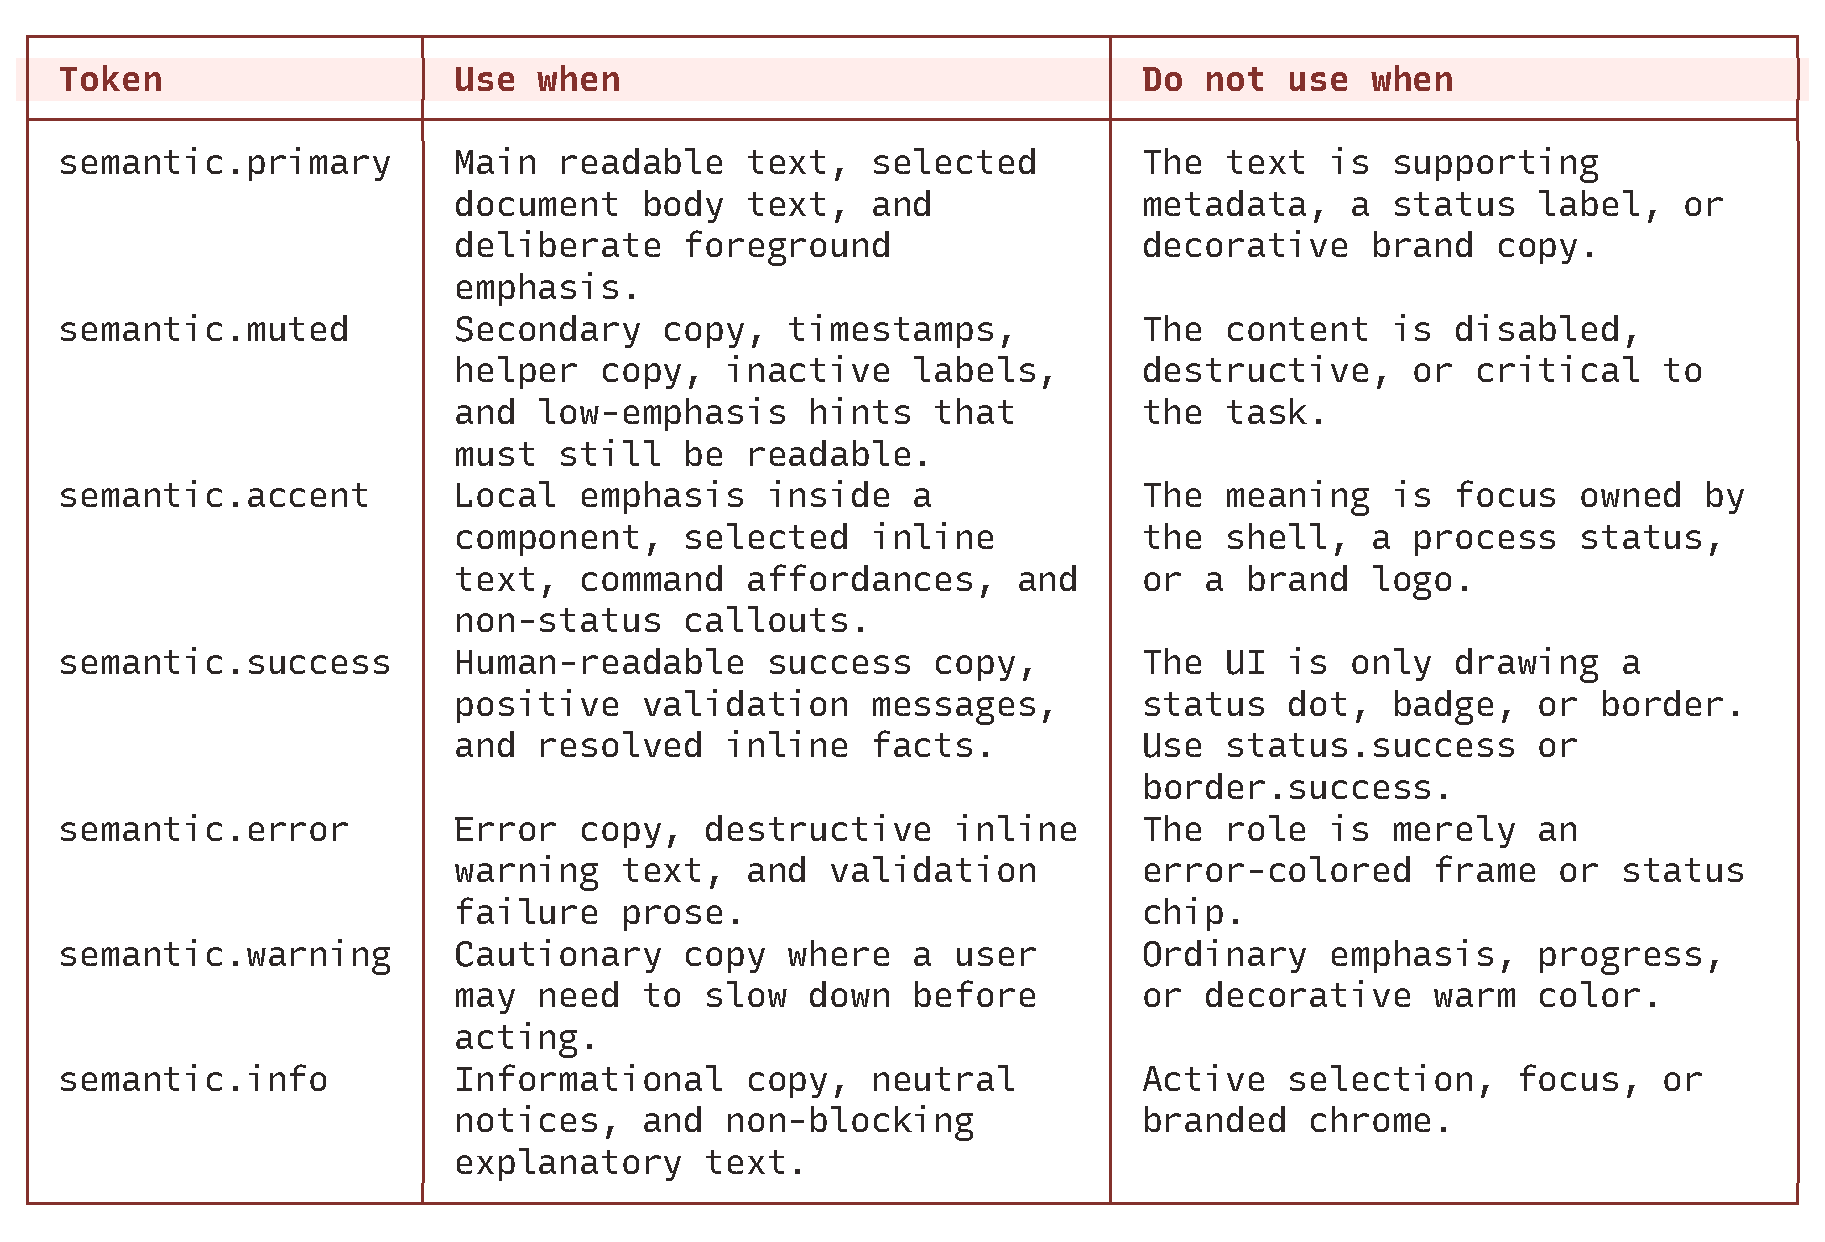
\includegraphics[width=\linewidth]{figures/tables/table-016-g1-1.pdf}
\par\smallskip{\scriptsize\color{BookMuted}Rows 1–7. Actual Bijou table component.}
\end{center}


\subsection{Surface Tokens}\label{record-028-surface-tokens}

\begin{center}
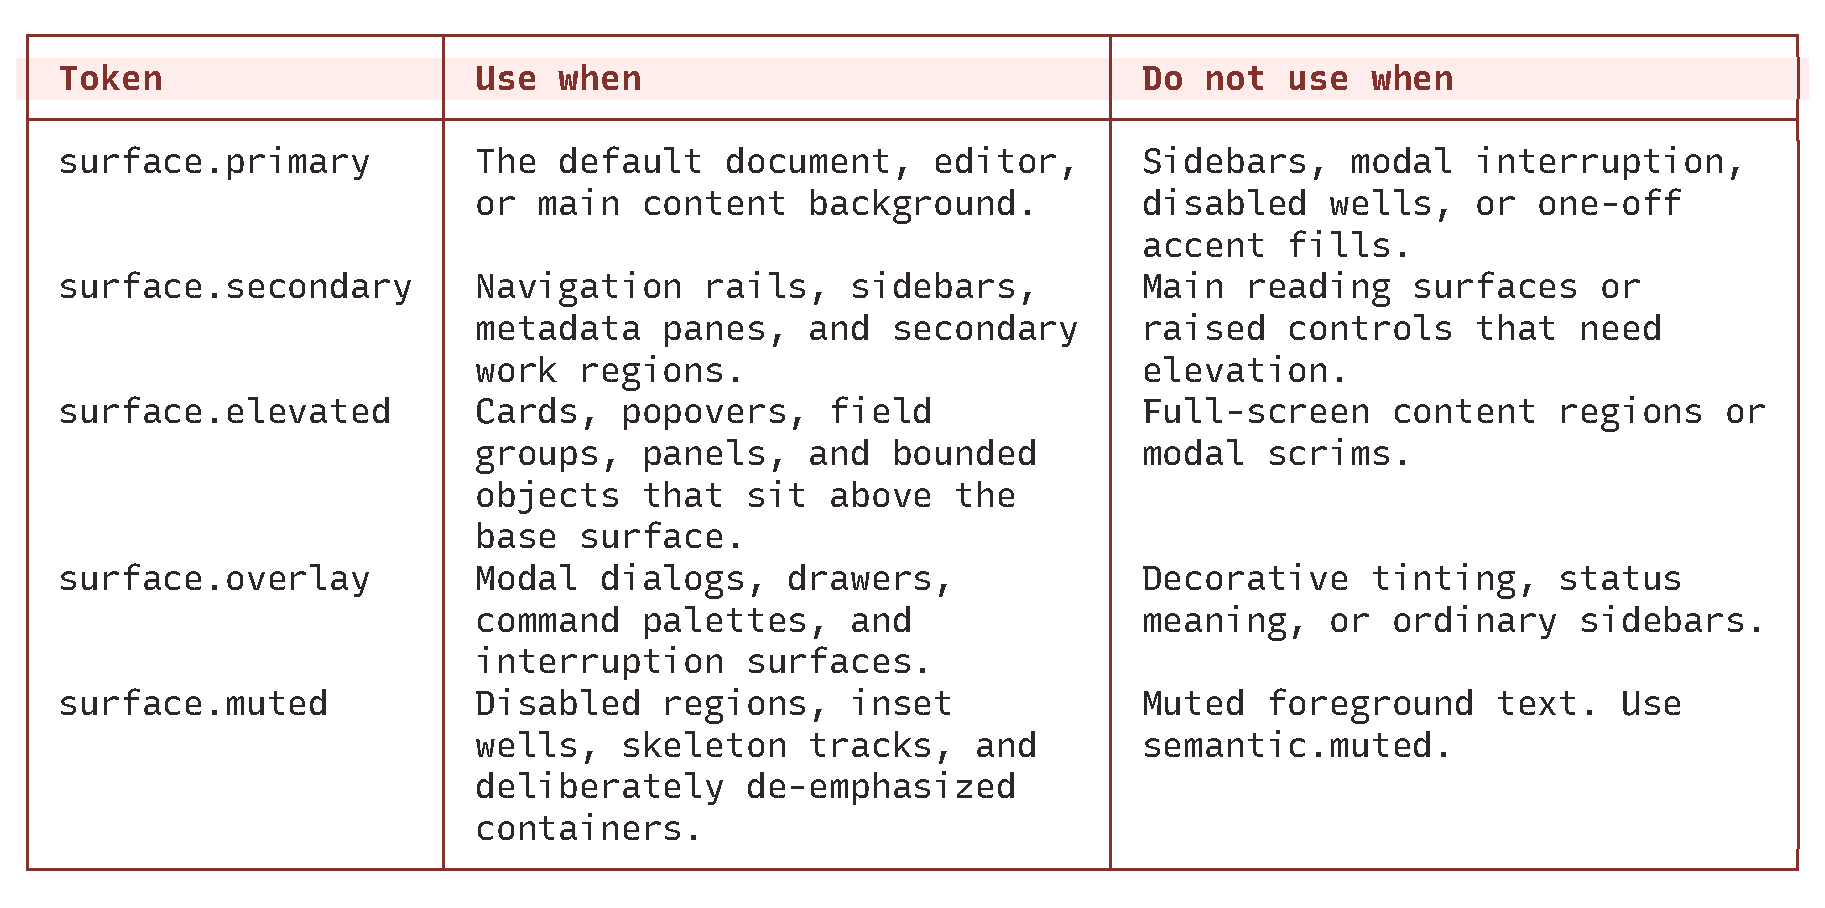
\includegraphics[width=\linewidth]{figures/tables/table-017-g1-1.pdf}
\par\smallskip{\scriptsize\color{BookMuted}Rows 1–5. Actual Bijou table component.}
\end{center}


\subsection{Border Tokens}\label{record-028-border-tokens}

\begin{center}
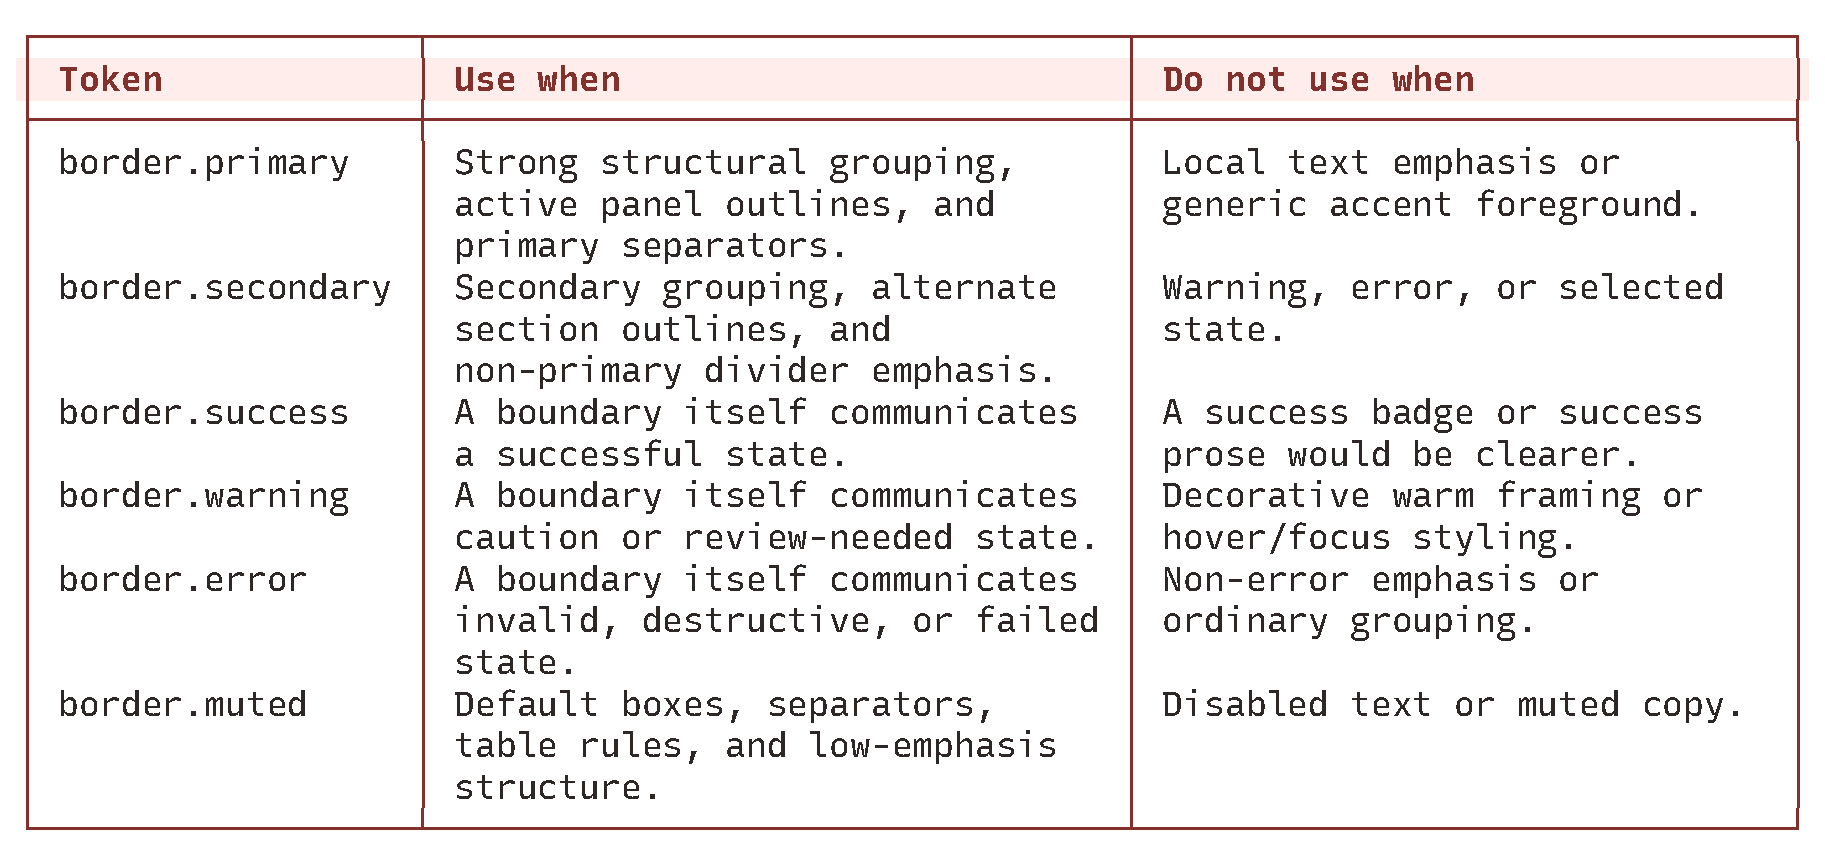
\includegraphics[width=\linewidth]{figures/tables/table-018-g1-1.pdf}
\par\smallskip{\scriptsize\color{BookMuted}Rows 1–6. Actual Bijou table component.}
\end{center}


\subsection{UI Tokens}\label{record-028-ui-tokens}

\begin{center}
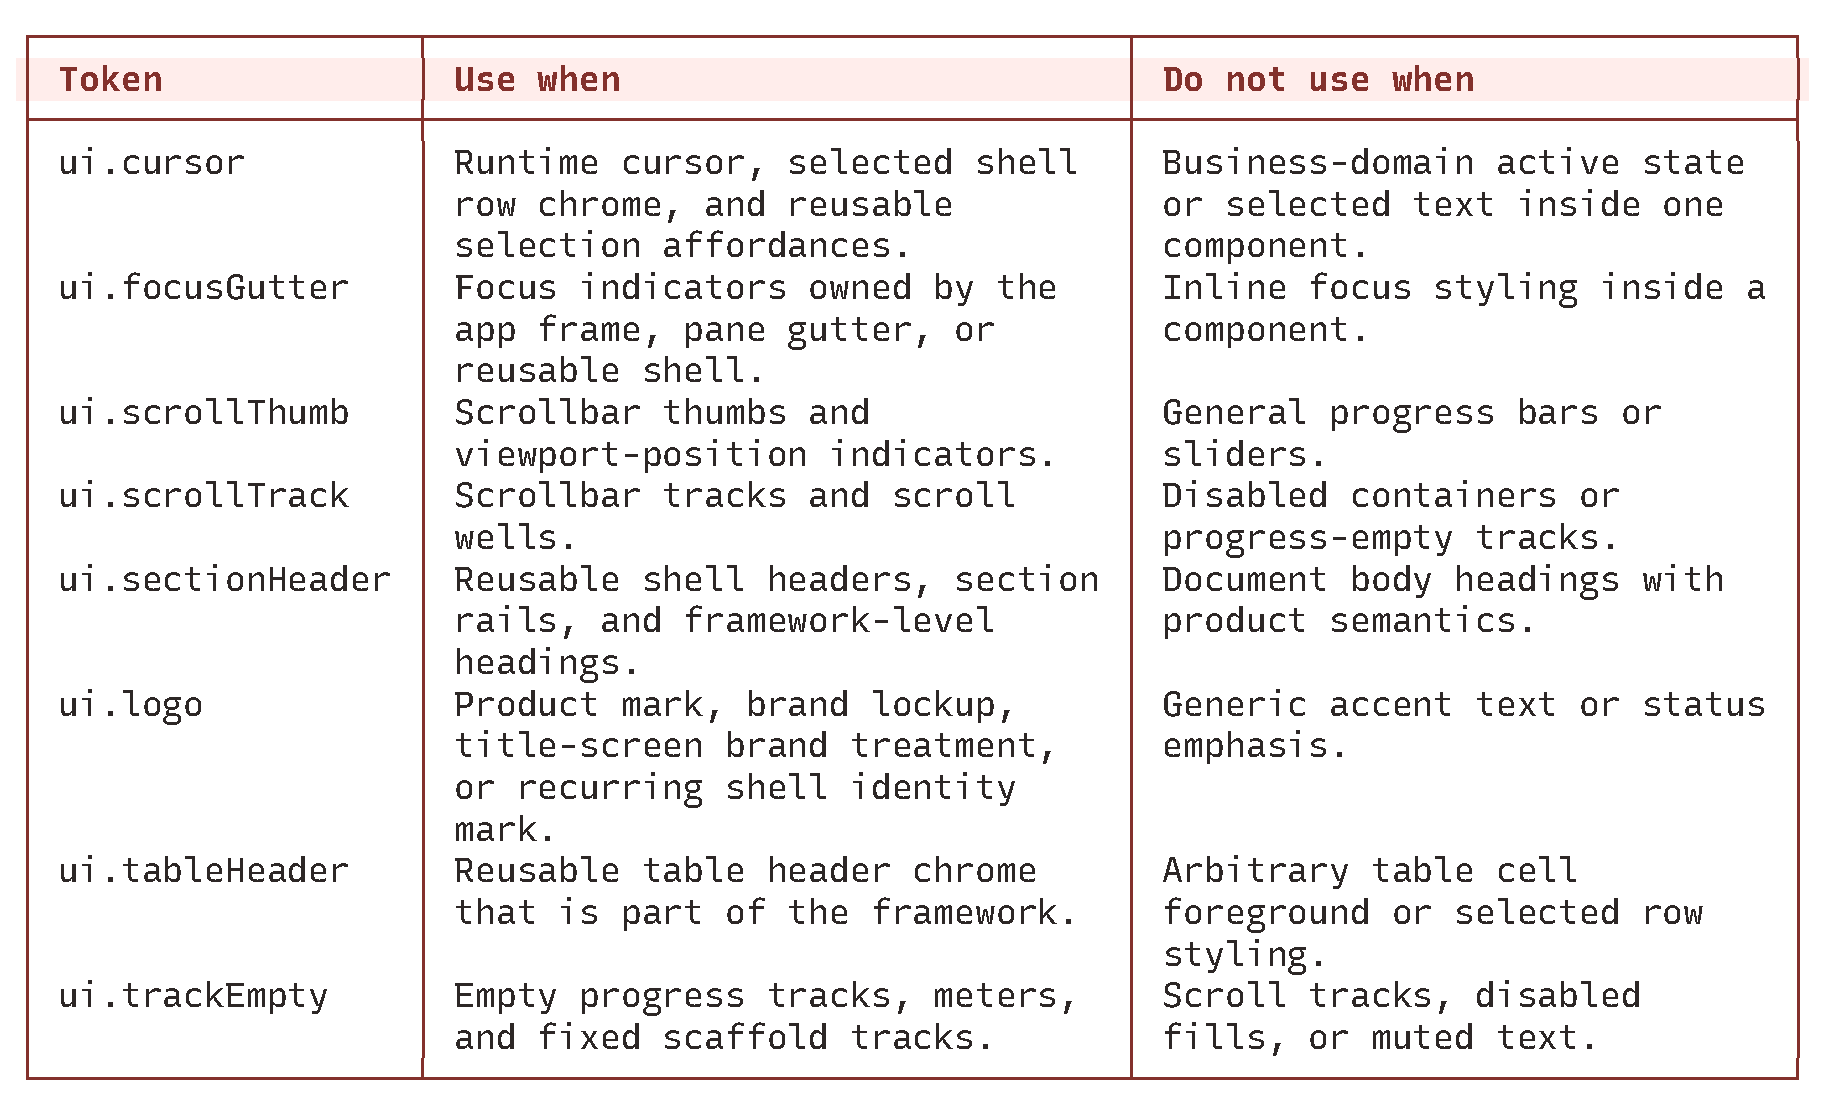
\includegraphics[width=\linewidth]{figures/tables/table-019-g1-1.pdf}
\par\smallskip{\scriptsize\color{BookMuted}Rows 1–8. Actual Bijou table component.}
\end{center}


\subsection{Status Tokens}\label{record-028-status-tokens}

\begin{center}
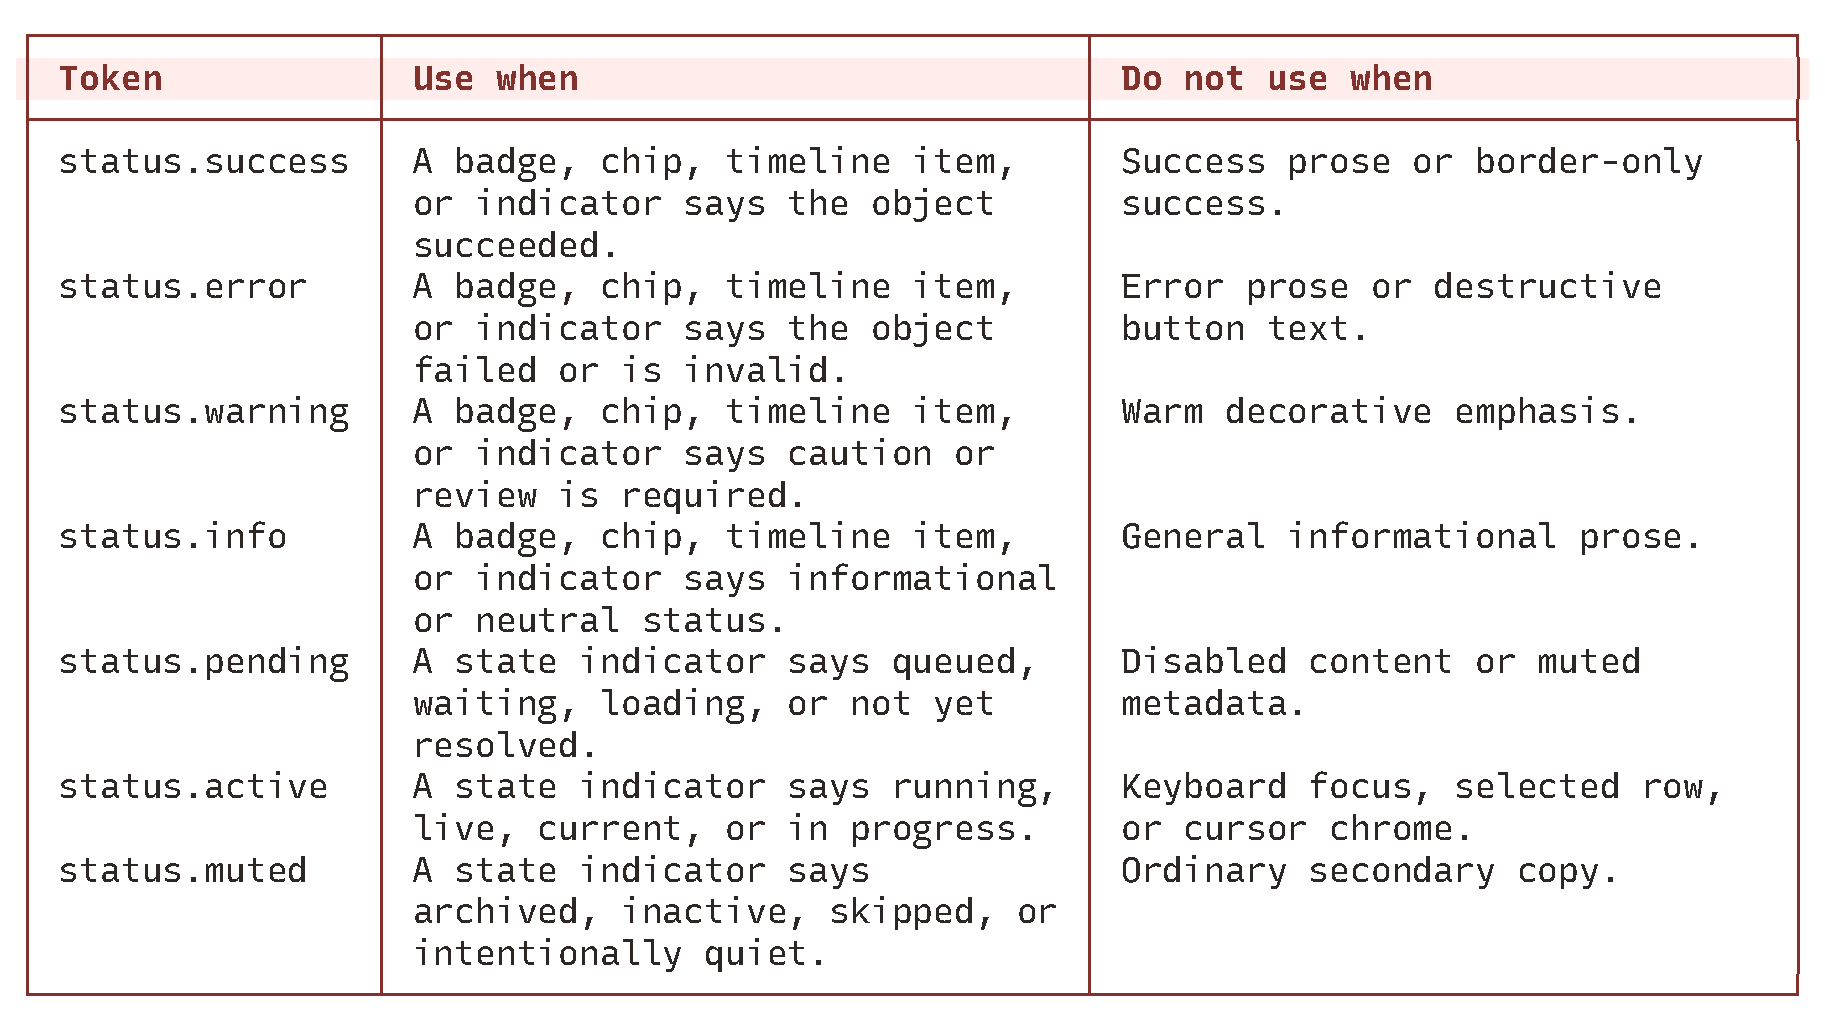
\includegraphics[width=\linewidth]{figures/tables/table-020-g1-1.pdf}
\par\smallskip{\scriptsize\color{BookMuted}Rows 1–7. Actual Bijou table component.}
\end{center}


\subsection{Gradient Tokens}\label{record-028-gradient-tokens}

\begin{center}
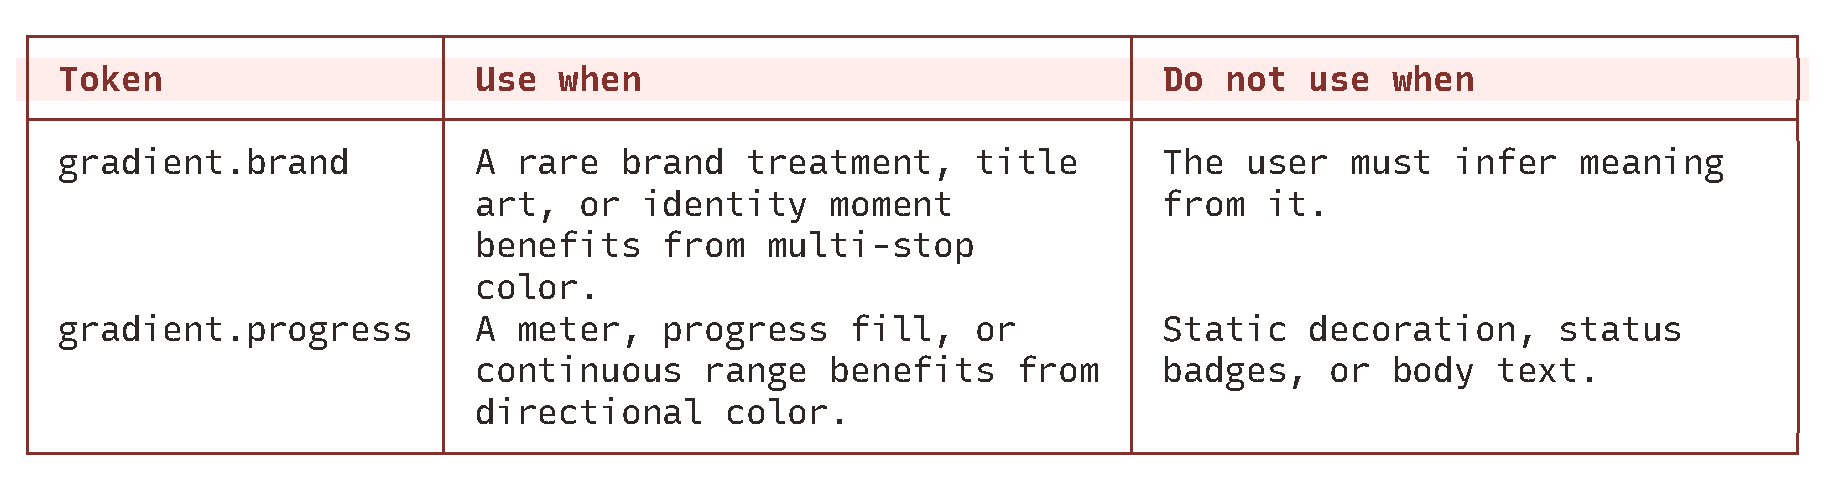
\includegraphics[width=\linewidth]{figures/tables/table-021-g1-1.pdf}
\par\smallskip{\scriptsize\color{BookMuted}Rows 1–2. Actual Bijou table component.}
\end{center}


\section{Default Dark/Light UX Audit}\label{record-028-default-darklight-ux-audit}

The legacy \texttt{C\allowbreak{}Y\allowbreak{}A\allowbreak{}N\allowbreak{}\_\allowbreak{}M\allowbreak{}A\allowbreak{}G\allowbreak{}E\allowbreak{}N\allowbreak{}T\allowbreak{}A} preset is useful as a vivid terminal-native preset, but it is not ideal as the model for dense product surfaces. It uses saturated terminal colors for many unrelated jobs: cyan appears as info, active state, cursor, scrollbar, logo, and primary border; magenta appears as accent, secondary border, and focus gutter. That makes the app energetic, but it also makes many regions compete at the same visual priority.

Bijou's first-party defaults now use a calmer shell posture:

\begin{itemize}
\tightlist
\item
  neutral surfaces carry most of the screen
\item
  one accent family carries local emphasis and shell selection
\item
  status colors remain distinct from focus and brand
\item
  muted text remains contrast-safe instead of merely dim
\item
  dark and light themes both satisfy readable foreground/background pairs
\end{itemize}

The \texttt{B\allowbreak{}I\allowbreak{}J\allowbreak{}O\allowbreak{}U\allowbreak{}\_\allowbreak{}D\allowbreak{}A\allowbreak{}R\allowbreak{}K} preset uses dark neutral surfaces, readable cool/warm accents, and separate success/warning/error/info colors. The \texttt{B\allowbreak{}I\allowbreak{}J\allowbreak{}O\allowbreak{}U\allowbreak{}\_\allowbreak{}L\allowbreak{}I\allowbreak{}G\allowbreak{}H\allowbreak{}T} preset uses light neutral surfaces with darker semantic colors instead of pastel foregrounds. DOGFOOD consumes those defaults directly as one \texttt{D\allowbreak{}O\allowbreak{}G\allowbreak{}F\allowbreak{}O\allowbreak{}O\allowbreak{}D} shell theme family with \texttt{D\allowbreak{}a\allowbreak{}r\allowbreak{}k} and \texttt{L\allowbreak{}i\allowbreak{}g\allowbreak{}h\allowbreak{}t} modes, so the docs app proves the same palette family that first-party components should treat as the baseline. Both modes target at least 4.5:1 contrast for surface text and common semantic foregrounds on every shell surface.

Compared with large design systems, Bijou is intentionally compact today. The runtime vocabulary has about thirty direct color-bearing slots plus two gradient roles. Material-style systems expose more paired foreground/background roles. Carbon and Atlassian-style systems go further with text hierarchy, interaction states, icon roles, and component-specific aliases. Bijou should grow only when a missing role causes repeated ambiguity in real components.

\section{Safe-Pair Contrast Contract}\label{record-028-safe-pair-contrast-contract}

Theme contrast is declared through safe pairs rather than buried inside one-off test loops. A safe pair names a foreground token path and a background token path that a theme promises will remain readable.

Safe-pair background paths may target token background slots:

\begin{CodeBlock}
semantic.primary on surface.primary.bg
semantic.muted on surface.secondary.bg
status.active on surface.overlay.bg
ui.cursor on surface.elevated.bg
\end{CodeBlock}

Use the \texttt{d\allowbreak{}e\allowbreak{}f\allowbreak{}i\allowbreak{}n\allowbreak{}e\allowbreak{}T\allowbreak{}h\allowbreak{}e\allowbreak{}m\allowbreak{}e\allowbreak{}S\allowbreak{}a\allowbreak{}f\allowbreak{}e\allowbreak{}P\allowbreak{}a\allowbreak{}i\allowbreak{}r\allowbreak{}s\allowbreak{}(\allowbreak{})} builder when a first-party app or component needs a reusable contrast matrix:

\begin{CodeBlock}
const pairs = defineThemeSafePairs()
  .readable('semantic.primary', 'surface.primary.bg')
  .status('status.error', 'surface.overlay.bg')
  .chrome('ui.cursor', 'surface.secondary.bg')
  .build();
\end{CodeBlock}

Then pass those pairs to \texttt{d\allowbreak{}o\allowbreak{}c\allowbreak{}t\allowbreak{}o\allowbreak{}r\allowbreak{}T\allowbreak{}h\allowbreak{}e\allowbreak{}m\allowbreak{}e\allowbreak{}(\allowbreak{})}:

\begin{CodeBlock}
const report = doctorTheme(theme, { contrastPairs: pairs });
\end{CodeBlock}

Safe-pair kinds communicate intent:

\begin{itemize}
\tightlist
\item
  \texttt{r\allowbreak{}e\allowbreak{}a\allowbreak{}d\allowbreak{}a\allowbreak{}b\allowbreak{}l\allowbreak{}e}: ordinary text or component foregrounds that must stay legible
\item
  \texttt{s\allowbreak{}t\allowbreak{}a\allowbreak{}t\allowbreak{}u\allowbreak{}s}: process, health, timeline, or object-state colors
\item
  \texttt{c\allowbreak{}h\allowbreak{}r\allowbreak{}o\allowbreak{}m\allowbreak{}e}: shell/runtime affordances such as cursor and selection chrome
\end{itemize}

Do not use safe pairs as a way to bless every possible token combination. Declare pairs only when a component or product surface expects that combination to work.

\section{Theme Debugger And Lab}\label{record-028-theme-debugger-and-lab}

DOGFOOD now has two inspectability surfaces:

\begin{itemize}
\tightlist
\item
  \texttt{F\allowbreak{}1\allowbreak{}0} opens a bounded Theme Inspector drawer in the docs shell.
\item
  The \texttt{T\allowbreak{}h\allowbreak{}e\allowbreak{}m\allowbreak{}e\allowbreak{}s} page publishes a Theme Lab with default palettes, shell-gallery facts, token swatches, and safe-pair diagnostics.
\end{itemize}

Current UX:

\begin{itemize}
\tightlist
\item
  \texttt{F\allowbreak{}1\allowbreak{}0} opens the drawer on the active DOGFOOD shell theme.
\item
  \texttt{F\allowbreak{}1\allowbreak{}0} or \texttt{E\allowbreak{}s\allowbreak{}c} closes the drawer.
\item
  The drawer shows token swatches grouped by \texttt{s\allowbreak{}e\allowbreak{}m\allowbreak{}a\allowbreak{}n\allowbreak{}t\allowbreak{}i\allowbreak{}c}, \texttt{s\allowbreak{}u\allowbreak{}r\allowbreak{}f\allowbreak{}a\allowbreak{}c\allowbreak{}e}, \texttt{b\allowbreak{}o\allowbreak{}r\allowbreak{}d\allowbreak{}e\allowbreak{}r}, \texttt{u\allowbreak{}i}, \texttt{s\allowbreak{}t\allowbreak{}a\allowbreak{}t\allowbreak{}u\allowbreak{}s}, and \texttt{g\allowbreak{}r\allowbreak{}a\allowbreak{}d\allowbreak{}i\allowbreak{}e\allowbreak{}n\allowbreak{}t}.
\item
  Each swatch renders the token path and uses the token value as the swatch fill or foreground depending on token family.
\item
  The drawer reports the safe-pair pass count for the active theme.
\item
  The Theme Lab page lists the first-party dark/light defaults, DOGFOOD shell themes, landing palette themes, and token swatches.
\end{itemize}

Still deferred:

\begin{itemize}
\tightlist
\item
  dark/light preview without committing the app theme
\item
  element-level token overlays
\item
  renderer provenance that can report whether a cell came from a token, raw color, or lowered/no-color fallback
\end{itemize}

The current implementation inspects theme tokens only. Element-level token overlays should wait until renderer provenance is available, because guessing token ownership from final RGB values would be misleading.

\section{First-Party Defaults}\label{record-028-first-party-defaults}

When first-party components need a default token and do not have stronger domain-specific semantics, prefer these defaults:

\begin{itemize}
\tightlist
\item
  default supporting text: \texttt{s\allowbreak{}e\allowbreak{}m\allowbreak{}a\allowbreak{}n\allowbreak{}t\allowbreak{}i\allowbreak{}c\allowbreak{}.\allowbreak{}m\allowbreak{}u\allowbreak{}t\allowbreak{}e\allowbreak{}d}
\item
  explicit primary emphasis: \texttt{s\allowbreak{}e\allowbreak{}m\allowbreak{}a\allowbreak{}n\allowbreak{}t\allowbreak{}i\allowbreak{}c\allowbreak{}.\allowbreak{}p\allowbreak{}r\allowbreak{}i\allowbreak{}m\allowbreak{}a\allowbreak{}r\allowbreak{}y}
\item
  local active or focused affordance inside a component: \texttt{s\allowbreak{}e\allowbreak{}m\allowbreak{}a\allowbreak{}n\allowbreak{}t\allowbreak{}i\allowbreak{}c\allowbreak{}.\allowbreak{}a\allowbreak{}c\allowbreak{}c\allowbreak{}e\allowbreak{}n\allowbreak{}t}
\item
  default structural border: \texttt{b\allowbreak{}o\allowbreak{}r\allowbreak{}d\allowbreak{}e\allowbreak{}r\allowbreak{}.\allowbreak{}m\allowbreak{}u\allowbreak{}t\allowbreak{}e\allowbreak{}d}
\item
  default contained-region fill: \texttt{s\allowbreak{}u\allowbreak{}r\allowbreak{}f\allowbreak{}a\allowbreak{}c\allowbreak{}e\allowbreak{}.\allowbreak{}e\allowbreak{}l\allowbreak{}e\allowbreak{}v\allowbreak{}a\allowbreak{}t\allowbreak{}e\allowbreak{}d}
\item
  default secondary-pane fill: \texttt{s\allowbreak{}u\allowbreak{}r\allowbreak{}f\allowbreak{}a\allowbreak{}c\allowbreak{}e\allowbreak{}.\allowbreak{}s\allowbreak{}e\allowbreak{}c\allowbreak{}o\allowbreak{}n\allowbreak{}d\allowbreak{}a\allowbreak{}r\allowbreak{}y}
\item
  default overlay fill: \texttt{s\allowbreak{}u\allowbreak{}r\allowbreak{}f\allowbreak{}a\allowbreak{}c\allowbreak{}e\allowbreak{}.\allowbreak{}o\allowbreak{}v\allowbreak{}e\allowbreak{}r\allowbreak{}l\allowbreak{}a\allowbreak{}y}
\item
  default disabled or inset fill: \texttt{s\allowbreak{}u\allowbreak{}r\allowbreak{}f\allowbreak{}a\allowbreak{}c\allowbreak{}e\allowbreak{}.\allowbreak{}m\allowbreak{}u\allowbreak{}t\allowbreak{}e\allowbreak{}d}
\item
  reusable shell cursor or selected-shell chrome: \texttt{u\allowbreak{}i\allowbreak{}.\allowbreak{}c\allowbreak{}u\allowbreak{}r\allowbreak{}s\allowbreak{}o\allowbreak{}r}
\item
  reusable focused shell gutter chrome: \texttt{u\allowbreak{}i\allowbreak{}.\allowbreak{}f\allowbreak{}o\allowbreak{}c\allowbreak{}u\allowbreak{}s\allowbreak{}G\allowbreak{}u\allowbreak{}t\allowbreak{}t\allowbreak{}e\allowbreak{}r}
\item
  reusable scrollbar chrome: \texttt{u\allowbreak{}i\allowbreak{}.\allowbreak{}s\allowbreak{}c\allowbreak{}r\allowbreak{}o\allowbreak{}l\allowbreak{}l\allowbreak{}T\allowbreak{}h\allowbreak{}u\allowbreak{}m\allowbreak{}b} and \texttt{u\allowbreak{}i\allowbreak{}.\allowbreak{}s\allowbreak{}c\allowbreak{}r\allowbreak{}o\allowbreak{}l\allowbreak{}l\allowbreak{}T\allowbreak{}r\allowbreak{}a\allowbreak{}c\allowbreak{}k}
\item
  table header chrome: \texttt{u\allowbreak{}i\allowbreak{}.\allowbreak{}t\allowbreak{}a\allowbreak{}b\allowbreak{}l\allowbreak{}e\allowbreak{}H\allowbreak{}e\allowbreak{}a\allowbreak{}d\allowbreak{}e\allowbreak{}r}
\item
  progress empty track: \texttt{u\allowbreak{}i\allowbreak{}.\allowbreak{}t\allowbreak{}r\allowbreak{}a\allowbreak{}c\allowbreak{}k\allowbreak{}E\allowbreak{}m\allowbreak{}p\allowbreak{}t\allowbreak{}y}
\end{itemize}

These defaults are conventions, not excuses to skip judgment. If a component has a stronger semantic job, use the family that matches the job.

\section{First-Party Prohibitions}\label{record-028-first-party-prohibitions}

First-party components should follow these rules:

\begin{itemize}
\tightlist
\item
  do not read raw token paths from \texttt{c\allowbreak{}t\allowbreak{}x\allowbreak{}.\allowbreak{}t\allowbreak{}h\allowbreak{}e\allowbreak{}m\allowbreak{}e\allowbreak{}.\allowbreak{}t\allowbreak{}h\allowbreak{}e\allowbreak{}m\allowbreak{}e\allowbreak{}.\allowbreak{}*} when an accessor exists
\item
  do not invent new first-party token families ad hoc
\item
  do not use \texttt{s\allowbreak{}t\allowbreak{}a\allowbreak{}t\allowbreak{}u\allowbreak{}s\allowbreak{}.\allowbreak{}*} when the real meaning is focus or selection
\item
  do not use \texttt{s\allowbreak{}u\allowbreak{}r\allowbreak{}f\allowbreak{}a\allowbreak{}c\allowbreak{}e\allowbreak{}.\allowbreak{}*} as a generic foreground-emphasis bucket
\item
  do not use gradients as a substitute for semantic color
\item
  do not rely on color alone; meaning must survive \texttt{n\allowbreak{}o\allowbreak{}C\allowbreak{}o\allowbreak{}l\allowbreak{}o\allowbreak{}r}, \texttt{p\allowbreak{}i\allowbreak{}p\allowbreak{}e}, and \texttt{a\allowbreak{}c\allowbreak{}c\allowbreak{}e\allowbreak{}s\allowbreak{}s\allowbreak{}i\allowbreak{}b\allowbreak{}l\allowbreak{}e}
\end{itemize}

If the current token families are not expressive enough, change the theme contract and docs in the same slice instead of sneaking around the vocabulary.

\section{Extension Rules}\label{record-028-extension-rules}

Third-party and app-level code may extend:

\begin{itemize}
\tightlist
\item
  \texttt{s\allowbreak{}t\allowbreak{}a\allowbreak{}t\allowbreak{}u\allowbreak{}s}
\item
  \texttt{u\allowbreak{}i}
\item
  \texttt{g\allowbreak{}r\allowbreak{}a\allowbreak{}d\allowbreak{}i\allowbreak{}e\allowbreak{}n\allowbreak{}t}
\end{itemize}

That is already part of the generic \texttt{T\allowbreak{}h\allowbreak{}e\allowbreak{}m\allowbreak{}e\allowbreak{}<\allowbreak{}S\allowbreak{},\allowbreak{} \allowbreak{}U\allowbreak{},\allowbreak{} \allowbreak{}G\allowbreak{}>} contract.

Rules for extension:

\begin{itemize}
\tightlist
\item
  extend when the new key represents a stable semantic role, not one component's temporary styling whim
\item
  keep first-party components on the built-in shared vocabulary unless the contract is intentionally widened
\item
  prefer wrapping a component with explicit token options over hard-coding raw token-path lookups
\item
  when theme changes must invalidate cached component work, prefer the public \texttt{o\allowbreak{}b\allowbreak{}s\allowbreak{}e\allowbreak{}r\allowbreak{}v\allowbreak{}e\allowbreak{}T\allowbreak{}h\allowbreak{}e\allowbreak{}m\allowbreak{}e\allowbreak{}(\allowbreak{}c\allowbreak{}t\allowbreak{}x\allowbreak{},\allowbreak{} \allowbreak{}h\allowbreak{}a\allowbreak{}n\allowbreak{}d\allowbreak{}l\allowbreak{}e\allowbreak{}r\allowbreak{})} seam over direct \texttt{t\allowbreak{}o\allowbreak{}k\allowbreak{}e\allowbreak{}n\allowbreak{}G\allowbreak{}r\allowbreak{}a\allowbreak{}p\allowbreak{}h\allowbreak{}.\allowbreak{}o\allowbreak{}n\allowbreak{}(\allowbreak{}.\allowbreak{}.\allowbreak{}.\allowbreak{})}
\end{itemize}

\section{Access Pattern}\label{record-028-access-pattern}

Component code should prefer the accessor layer:

\begin{itemize}
\tightlist
\item
  \texttt{c\allowbreak{}t\allowbreak{}x\allowbreak{}.\allowbreak{}s\allowbreak{}e\allowbreak{}m\allowbreak{}a\allowbreak{}n\allowbreak{}t\allowbreak{}i\allowbreak{}c\allowbreak{}(\allowbreak{}.\allowbreak{}.\allowbreak{}.\allowbreak{})}
\item
  \texttt{c\allowbreak{}t\allowbreak{}x\allowbreak{}.\allowbreak{}s\allowbreak{}u\allowbreak{}r\allowbreak{}f\allowbreak{}a\allowbreak{}c\allowbreak{}e\allowbreak{}(\allowbreak{}.\allowbreak{}.\allowbreak{}.\allowbreak{})}
\item
  \texttt{c\allowbreak{}t\allowbreak{}x\allowbreak{}.\allowbreak{}b\allowbreak{}o\allowbreak{}r\allowbreak{}d\allowbreak{}e\allowbreak{}r\allowbreak{}(\allowbreak{}.\allowbreak{}.\allowbreak{}.\allowbreak{})}
\item
  \texttt{c\allowbreak{}t\allowbreak{}x\allowbreak{}.\allowbreak{}s\allowbreak{}t\allowbreak{}a\allowbreak{}t\allowbreak{}u\allowbreak{}s\allowbreak{}(\allowbreak{}.\allowbreak{}.\allowbreak{}.\allowbreak{})}
\item
  \texttt{c\allowbreak{}t\allowbreak{}x\allowbreak{}.\allowbreak{}u\allowbreak{}i\allowbreak{}(\allowbreak{}.\allowbreak{}.\allowbreak{}.\allowbreak{})}
\item
  \texttt{c\allowbreak{}t\allowbreak{}x\allowbreak{}.\allowbreak{}g\allowbreak{}r\allowbreak{}a\allowbreak{}d\allowbreak{}i\allowbreak{}e\allowbreak{}n\allowbreak{}t\allowbreak{}(\allowbreak{}.\allowbreak{}.\allowbreak{}.\allowbreak{})}
\end{itemize}

That keeps component code coupled to the public vocabulary instead of the raw object shape or token-graph internals.

\section{Relationship To Foundations}\label{record-028-relationship-to-foundations}

The design-system foundations describe the high-level visual roles:

\begin{itemize}
\tightlist
\item
  foreground
\item
  surface
\item
  status
\item
  accent
\item
  border or separator
\end{itemize}

This page maps those roles onto the shipped API vocabulary:

\begin{itemize}
\tightlist
\item
  foreground -\textgreater{} \texttt{s\allowbreak{}e\allowbreak{}m\allowbreak{}a\allowbreak{}n\allowbreak{}t\allowbreak{}i\allowbreak{}c}
\item
  accent -\textgreater{} \texttt{s\allowbreak{}e\allowbreak{}m\allowbreak{}a\allowbreak{}n\allowbreak{}t\allowbreak{}i\allowbreak{}c\allowbreak{}.\allowbreak{}a\allowbreak{}c\allowbreak{}c\allowbreak{}e\allowbreak{}n\allowbreak{}t}
\item
  surface -\textgreater{} \texttt{s\allowbreak{}u\allowbreak{}r\allowbreak{}f\allowbreak{}a\allowbreak{}c\allowbreak{}e}
\item
  border or separator -\textgreater{} \texttt{b\allowbreak{}o\allowbreak{}r\allowbreak{}d\allowbreak{}e\allowbreak{}r}
\item
  reusable framework chrome -\textgreater{} \texttt{u\allowbreak{}i}
\item
  explicit named state -\textgreater{} \texttt{s\allowbreak{}t\allowbreak{}a\allowbreak{}t\allowbreak{}u\allowbreak{}s}
\item
  rare multi-stop emphasis -\textgreater{} \texttt{g\allowbreak{}r\allowbreak{}a\allowbreak{}d\allowbreak{}i\allowbreak{}e\allowbreak{}n\allowbreak{}t}
\end{itemize}

\section{Examples}\label{record-028-examples}

Examples of the intended split:

\begin{itemize}
\tightlist
\item
  \texttt{a\allowbreak{}l\allowbreak{}e\allowbreak{}r\allowbreak{}t\allowbreak{}(\allowbreak{})} should use \texttt{s\allowbreak{}e\allowbreak{}m\allowbreak{}a\allowbreak{}n\allowbreak{}t\allowbreak{}i\allowbreak{}c\allowbreak{}(\allowbreak{}v\allowbreak{}a\allowbreak{}r\allowbreak{}i\allowbreak{}a\allowbreak{}n\allowbreak{}t\allowbreak{})} plus a matching border, not a gradient
\item
  \texttt{b\allowbreak{}a\allowbreak{}d\allowbreak{}g\allowbreak{}e\allowbreak{}(\allowbreak{})} should use \texttt{s\allowbreak{}t\allowbreak{}a\allowbreak{}t\allowbreak{}u\allowbreak{}s\allowbreak{}.\allowbreak{}*} when it is carrying a real status
\item
  \texttt{k\allowbreak{}b\allowbreak{}d\allowbreak{}(\allowbreak{})} should use muted structure tokens, not a status token
\item
  \texttt{t\allowbreak{}a\allowbreak{}b\allowbreak{}l\allowbreak{}e\allowbreak{}S\allowbreak{}u\allowbreak{}r\allowbreak{}f\allowbreak{}a\allowbreak{}c\allowbreak{}e\allowbreak{}(\allowbreak{})} should use \texttt{u\allowbreak{}i\allowbreak{}.\allowbreak{}t\allowbreak{}a\allowbreak{}b\allowbreak{}l\allowbreak{}e\allowbreak{}H\allowbreak{}e\allowbreak{}a\allowbreak{}d\allowbreak{}e\allowbreak{}r} for reusable header chrome
\item
  shell cursor, focused gutters, scrollbars, and track fills should use \texttt{u\allowbreak{}i\allowbreak{}.\allowbreak{}*}, not business statuses
\item
  overlays and drawers should communicate interruption primarily through \texttt{s\allowbreak{}u\allowbreak{}r\allowbreak{}f\allowbreak{}a\allowbreak{}c\allowbreak{}e\allowbreak{}.\allowbreak{}o\allowbreak{}v\allowbreak{}e\allowbreak{}r\allowbreak{}l\allowbreak{}a\allowbreak{}y}, not by tinting everything as a warning
\end{itemize}

